\documentclass{article}

\textwidth=6.5in
\textheight=8.5in
\voffset=-54pt
\oddsidemargin=0in
\evensidemargin=0in
\setlength{\parskip}{8pt}
\setlength{\parindent}{0pt}

\usepackage{workbook}

\usepackage[sols]{handout}

\begin{document}

\htitle{Math Mb Final Review Session - Integration}

\begin{framed}
\textbf{The Definite Integral} When $a$ and $b$ are constants, the definite integral $\displaystyle \int_a^b f(t)\,dt$ equals some number that we can interpret in three ways:
    \begin{itemize}
        \item By definition, $\displaystyle \int_a^b f(t)\,dt$ is the limit of a Riemann sum of $n$ slices as $n \to \infty$: 
        \[ \lim_{n \to \infty} \underbrace{\sum_{k=1}^n f(x_k)\, \Delta x}_{R_n}
    = \lim_{n \to \infty} \underbrace{\sum_{k=0}^{n-1} f(x_k)\, \Delta
      x}_{L_n}, \text{ where } \Delta x = \frac{b - a}{n} \text{ and } x_k
    = a + k \Delta x\]
    \vspace{-17pt}
        \item If $a<b$, we can visualize $\displaystyle \int_a^b f(t)\,dt$ graphically as $\fitb{2.5in}{\text{\textcolor{red}{the signed area between $f(t)$ and the}}}$
        \newline
        \newline
        $\fitb{5.6in}{\text{\textcolor{red}{horizontal axis between $t=a$ and $t=b$}}}$
        \newline
        \item In the case that $f(t)$ is a rate function, then $\displaystyle \int_a^b f(t)\,dt$ is $\fitb{2.2in}{\text{\textcolor{red}{the net change in an amount}}}$
        \newline
        \newline
        $\fitb{5.6in}{\text{\textcolor{red}{between $t=a$ and $t=b$, or the accumulation of some amount between $t=a$ and $t=b$}}}$
    \end{itemize}
    \end{framed}

\begin{framed}
  \vspace{0.05in}
   \textbf{The Fundamental Theorem of Calculus}
  \begin{itemize}
  \item The function $A(x) = \displaystyle \int_a^x
  f(t)\,dt$ outputs the \textit{area} 
  between $f(t)$ and the horizontal axis from the \newline
      \vfill
      anchor $t=a$ to the variable upper bound $t=x$.
      \item The FTOC Part 1 states that, if $f(t)$ is a continuous function, then $\dfrac{d}{dx}A(x) = \fitb{1.1in}{\textcolor{red}{f(x)}}$.\newline
      \vfill
      We can also write this as $A'(x)=\fitb{1.4in}{\textcolor{red}{f(x)}}$ or $\dfrac{d}{dx}\displaystyle \int_a^x
  f(t)\,dt = \fitb{1.4in}{\textcolor{red}{f(x)}}$.
      \newline
      \vfill
      \item The FTOC Part 2 states that, if $f$ is
  a continuous function on $[a, b]$ and $F$ is an \textbf{antiderivative} of \newline \vfill  $f$,
  that is, $F'=f$, then $\displaystyle \int_a^b f(t)\,dt
  = {}$ \fitb{3.6in}{$\bm{\textcolor{red}{F(b)-F(a)}}$}. 
  \vfill
  \end{itemize}
  \end{framed}

\begin{enumerate}
  
\item What are some strategies for evaluating definite and indefinite integrals?
\probonly{\vfill}

\begin{solution}
\begin{itemize}
    \item basic antiderivatives
    \item basic geometry (definite integrals)
    \item properties of integrals
    \item integration by substitution
    \item integration by parts
\end{itemize}
\end{solution}

\probonly{\newpage}

Compute the following definite integrals 

  \begin{enumerate}
      \item $\displaystyle \int_{-\pi}^\pi \left( \frac{3x^4 }{\pi} + 10\cos x +
      \frac{1}{e^x} \right) dx$
      
      \begin{solution}
        $\displaystyle \frac{3x^5}{5 \pi} + 10 \sin x - e^{-x} + C$.  Rewrite the third term in the integrand as $e^{-x}$ before integrating.  
    \end{solution}
    \probonly{\vfill}
  
  \item

  $\displaystyle \int_{-3}^{3} | 2x - 4| \, dx$

  \begin{solution}
    26.  Use geometry.
  \end{solution}
  \probonly{\vfill}


\item 

  $\displaystyle\int_1^{e} x^2\ln x \, dx$

  \begin{solution}
    $\dfrac{2e^3}{9}+\dfrac{1}{9}$. Use integration by parts with $u=\ln x$ and $dv = x^2\, dx$.
  \end{solution}
  \probonly{\vfill}

\item

  \begin{problem}
    $\displaystyle \int_0^{2\pi} \sin(2x - 4)\,dx$      
  \end{problem}

  \begin{solution}
    $\displaystyle - \frac{1}{2} \cos (4\pi - 4)+ \frac{1}{2} \cos (- 4)$.  Substitute $u = 2x -
    4$. 
  \end{solution}
  \probonly{\vfill}


\item

  \begin{problem}
    $\displaystyle \int_0^{\pi/2} \cos \left(3x - \frac{\pi}{2}
    \right)\,dx$ 
  \end{problem}

  \begin{solution}
    $\displaystyle \frac{1}{3}$.  Substitute $u = 3x - \frac{\pi}{2}$. 
  \end{solution}
  \probonly{\vfill}

  \probonly{\newpage}

\item

  \begin{problem}
    $\displaystyle \int_1^4 \frac{3x+1}{\sqrt{x}}\, dx$
  \end{problem}

  \begin{solution}
    $16$.  Expand the integrand. 
  \end{solution}
  \probonly{\vfill}

\item

  \begin{problem}
    $\displaystyle \int_1^{4} \frac{x}{3 \sqrt{x+1}} \, dx $
  \end{problem}

  \begin{solution}
    $\displaystyle \frac{2 \sqrt{2}}{9} + \frac{4 \sqrt{5}}{9}$.
    Substitute $u = x + 1$. 
  \end{solution}
  \probonly{\vfill}

\item

  \begin{problem}
    $\displaystyle \int_{0}^1 \frac{x+3}{(x^2 + 6x + 1)^3} \,dx$
  \end{problem}

  \begin{solution}
    $\displaystyle \frac{63}{256}$.  Substitute $u = x^2 + 6x + 1$. 
  \end{solution}
  \probonly{\vfill}

\item

  \begin{problem}
    $\displaystyle \int_{-2}^1 x \cdot 2^{x^2}\,dx$
  \end{problem}

  \begin{solution}
    $\displaystyle - \frac{7}{\ln 2}$.  Substitute $u = x^2$. 
  \end{solution}
  \probonly{\vfill}

\item

  \begin{problem}
    $\displaystyle \int_{-\pi/3}^{\pi/3} \left( 2|x| + \cos x \right)\,dx$
  \end{problem}

  \begin{solution}
    $\dfrac{2 \pi^2}{9} + \sqrt{3}$.  Split into a sum of two integrals;
    use geometry on the first.
  \end{solution}
  \probonly{\vfill}


\end{enumerate}

\probonly{\newpage}
  
  \begin{framed}
  \vspace{0.05in}
\textbf{Antiderivatives} An antiderivative of $f(x)$ is a function whose derivative is $f(x)$. If $F'(x)=f(x)$, the family of antiderivatives of $f(x)$ takes the form $F(x)+C$, since the derivative of the constant $C$ is $0$. This family of functions is given by the indefinite integral $\displaystyle \int f(x)\,dx$. 
    \vfill
    \begin{itemize}
    \item Common indefinite integrals include:

\begin{multicols}{2}
 $\displaystyle \int 1\,du\ =$
 \solonly{\textcolor{red}{$u+C$}}
 \newline
 
$\displaystyle \int \dfrac{1}{\sqrt{1-u^2}}\,du\ =$
\solonly{\textcolor{red}{$\arcsin u+C$}}
\newline
 
$\displaystyle \int \dfrac{1}{1+u^2}\,du\ =$
\solonly{\textcolor{red}{$\arctan u+C$}}
\newline

 $\displaystyle \int e^u\,du\ =$
 \solonly{\textcolor{red}{$e^u+C$}}
 \newline 
 
 $\displaystyle \int b^u\,du\ =$\probonly{\hspace{0.9in}, where $b>0$ and $b\neq1$}
\solonly{\textcolor{red}{$\dfrac{b^{u}}{\ln b}+C$, where $b>0$}}
\newline

$\displaystyle \int \cos(u)\,du\ =$
\solonly{\textcolor{red}{$\sin u+C$}}
\newline

$\displaystyle \int u^n\,du\ =$\probonly{\hspace{1.2in}, where $n\neq -1$}
\solonly{\textcolor{red}{$\dfrac{u^{n+1}}{n+1}+C$, where $n\neq -1$}}
\newline

$\displaystyle \int \sin(u)\,du\ =$
\solonly{\textcolor{red}{$-\cos u +C$}}
\newline

$\displaystyle \int \sec^2(u)\,du\ =$
\solonly{\textcolor{red}{$\tan u +C$}}
\newline

$\displaystyle \int \sec(u) \tan(u)\,du\ =$
\solonly{\textcolor{red}{$\sec u +C$}}
\newline 

$\displaystyle \int \dfrac{1}{u}\,du\ =$
\solonly{\textcolor{red}{$\ln |u| +C$}}
\newline
\newline
\newline

\end{multicols}

\end{itemize}
\end{framed}

\item Compute the following indefinite integrals
    
    \begin{enumerate}
        \item $\displaystyle \int 2x e^{x^2}\,dx$
        
        \begin{solution}
          $\displaystyle \int 2x e^{x^2}\,dx =e^{x^2} + C$. Use substitution with $u=x^2$.
        \end{solution}
        \probonly{\vfill}
        
        \item $\displaystyle \int \cos(x) \cos(\sin(x))\,dx$
        
        \begin{solution}
          $\displaystyle \int \cos(x) \cos(\sin(x))\,dx = \sin(\sin(x)) + C$. Use substitution with $u=\sin x$
        \end{solution}
        \probonly{\vfill}
        
        \item $\displaystyle \int \dfrac{x}{\sqrt{1-x^2}}\,dx$
        
        \begin{solution}
          $= - \sqrt{1 - x^2} + C$. Use substitution with $u=1-x^2$.
        \end{solution}
        \probonly{\vfill}
        
        \item $\displaystyle \int \dfrac{x^2 + x}{x^2}\,dx$
        
        \begin{solution}
          $\displaystyle \int \dfrac{x^2 + x}{x^2}\,dx = \int \dfrac{x^2}{x^2} + \dfrac{x}{x^2} \; dx = \int 1 + \dfrac{1}{x} \; dx = x + \ln|x| + C$ 
        \end{solution}
        \probonly{\vfill}
        
        \probonly{\newpage}
        
        \item $\displaystyle \int \dfrac{dx}{x\ln(x)}$
        
        \begin{solution}
          Let $u=\ln(x)$. Then $du = \dfrac{1}{x}$ and we have that this integral is 
          $$\displaystyle \int \dfrac{dx}{x\ln(x)} = \int \dfrac{1}{\ln(x)} \cdot \dfrac{1}{x} \cdot dx = \int \dfrac{1}{u} du = \ln|\ln(x)| + C$$
        \end{solution}
        \probonly{\vfill}
        
        \item $\displaystyle \int (\sin^2(x) + \cos^2(x))\,dx$
        
        \begin{solution}
          $\displaystyle \int (\sin^2(x) + \cos^2(x))\,dx = \int 1 \; dx$, as $\sin^2(x) = \cos^2(x) = 1$. So this is $\displaystyle \int dx = x + C$
        \end{solution}
        \probonly{\vfill}
        
        \item $\displaystyle \int x\cos(-4x)\,dx$
        
        \begin{solution}
          $-\dfrac{1}{4}\sin(-4x)-\dfrac{1}{16}\cos(-4x)+C$. Integration by parts with $u=x$ and $dv=\cos (-4x)\,dx$
        \end{solution}
        \probonly{\vfill}
        
        \item $\displaystyle \int 3x^{-1}\,dx$
        
        \begin{solution}
          $\displaystyle \int 3x^{-1}\,dx. = \int \dfrac{3}{x} \; dx = 3 \int \dfrac{1}{x} \; dx = 3 \ln|x| + C.$
        \end{solution}
        \probonly{\vfill}

        \item $\displaystyle\int \arctan\left(\dfrac{1}{x}\right)\, dx$
        
        \begin{solution}
            $x\arctan\left(\dfrac{1}{x}\right)+\dfrac{1}{2}\ln\left|1+x^2\right|+C$. First use integration by parts with $u=\arctan\left(\dfrac{1}{x}\right)$ and $dv=dx$. Then part of the solution involves evaluating $\displaystyle\int \dfrac{-x}{1+x^2} \, dx$. Use substitution with $w=1+x^2$.
        \end{solution}
        \vfill

\newpage
\item 
  
    % \savebox{\graph}{
    %   \begin{tikzpicture}
    %     \begin{axis}[gridgraph, xtick={-2, 0, ..., 12}, minor xtick={-1,
    %         1, ..., 11}, grid=both, minor ytick={-12, -10, ..., 12}, 
    %       ytick={-12, -8, ..., 12}, width=3.25in, height=2.5in,
    %       every axis plot/.style={no marks, very thick} ]          
    %       \addplot+[domain=-2:1] {-6*x-6};
    %       \addplot+[domain=1:5] {6*(x-1)-12};
    %       \addplot+[domain=5:7] {12};
    %       \addplot+[domain=7:12] {-3*(x-11)};
    %     \end{axis}
    %   \end{tikzpicture}
    % }

    Suppose that there was a flu epidemic in March in Boston, and the
    function $f(t)$ whose graph is shown below represents the \emph{rate of
      change} of the number of flu patients hospitalized at Massachusetts
    General Hospital, in people per day, where $t$ is measured in days and
    $t = 0$ represents noon on March 10.  (So, $t = -1$ is noon on March 9
    and $t = 1$ is noon on March 11.)  At noon on March 12, the hospital had
    60 flu patients.

      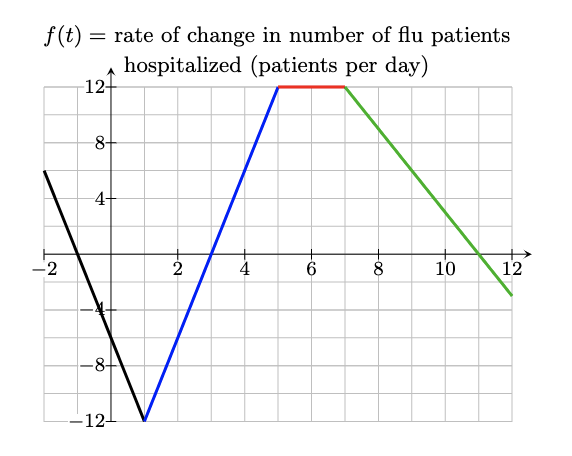
\includegraphics[scale=0.7]{flu_graph.png}

      \begin{enumerate}
          \item
      \begin{problem}[\vfill]
        How many flu patients were hospitalized at noon on March 13?
        (Please simplify your answer.)
      \end{problem}

      \begin{solution}
        At noon on March 12 ($t = 2$), the hospital had 60 flu patients.
        Between March 12 and March 13 ($t = 3$) , the net change in the
        number of flu patients was $\displaystyle \int_2^3 f(t)\,dt$.  So,
        the total number of patients hospitalized on March 13 was $60 +
        \displaystyle \int_2^3 f(t)\,dt$.  By interpreting the definite
        integral $\displaystyle \int_2^3 f(t)\,dt$ as a signed area, we see
        that it is equal to $-3$, so $60 + \displaystyle \int_2^3 f(t)\,dt =
        \boxed{57}$.
      \end{solution}

    \item
      \begin{problem}[\vfill]      
        At what times in $(-2, 12)$ was the number of patients in the
        hospital increasing?
      \end{problem}

      \begin{solution}
        The number of patients is increasing exactly when $f(t)$, the rate
        of change in the number of patients, is positive.  This happens on
        \fbox{$(-2, -1)$ and $(3, 11)$}.
      \end{solution}

    \item
      \begin{problem}[\vfill]
        At what time in $[-2, 12]$ was the number of hospitalized patients
        the highest?  How many patients were hospitalized at that time? 
      \end{problem}

      \begin{solution}
        In part b, we found that the number of
        patients is increasing on $(-2, -1)$ and $(3, 11)$ (and decreasing
        otherwise).  So, the number of patients must be greatest either at
        $t = -1$ or $t = 11$.  The net change in the number of patients
        between $t = -1$ and $t = 11$ is $\displaystyle \int_{-1}^{11}
        f(t)\,dt$, which is positive (we can see this by looking at the graph
        of $f(t)$), which means there are more patients at $\boxed{t =
          11}$.

        We are asked to find the number of patients hospitalized at that
        time, $t = 11$; by the same reasoning as in
        part a, it is $60 + \displaystyle
        \int_2^{11} f(t)\,dt$.  By interpreting the integral as signed area,
        we find that this is equal to $60 + 57 = \boxed{117}$ patients. 
      \end{solution}

    \item
      \begin{problem}[\vfill]
        At what time in $[-2, 12]$ was the number of hospitalized patients
        the lowest?  
      \end{problem}

      \begin{solution}
        In part b, we found that the number of
        patients is increasing on $(-2, -1)$ and $(3, 11)$ (and decreasing
        otherwise).  So, the number of patients must be lowest at $t = -2$,
        $t = 3$, or $t = 12$.  From $t = -2$ to $t = 3$, there is a net
        decrease in the number of patients (the signed area under $f$ from
        $-2$ to $3$ is negative), so the number of patients is lower at $t =
        3$ than at $t = -2$.  From $t = 3$ to $t = 12$, there is a net
        increase in the number of patients, so the number of patients is
        lowest at $\boxed{t = 3}$.
      \end{solution}
      
\end{enumerate}

\probonly{\newpage}

\item 

  The rate $r(t)$ at which liquid nitrogen is pumped in and out of a tank is
  shown in the graph below.  There are 30 cubic feet of liquid nitrogen in
  the tank at $t = 0$. Give exact answers to the following questions,
  using definite integrals where necessary. If your answer contains a
  definite integral, give an approximation.
  \begin{center}
    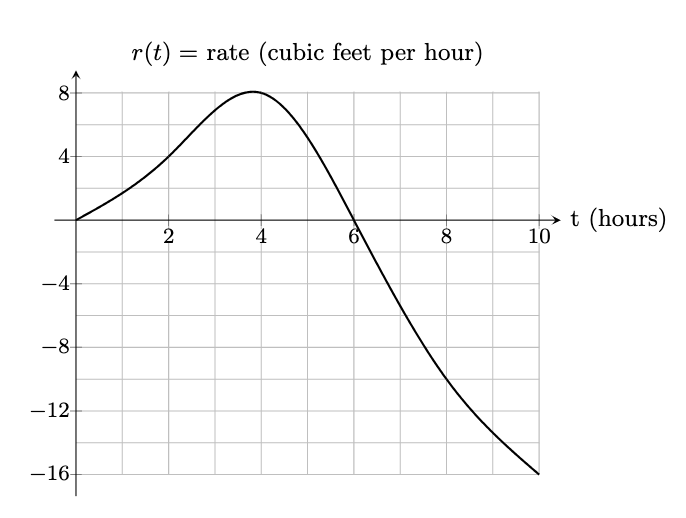
\includegraphics[scale=0.6]{nitrogen_graph.png}  
  \end{center}

  \begin{enumerate}
  \item
    \begin{problem}
      How much liquid nitrogen flows into the tank between $t=2$ and $t=3$?
    \end{problem}

    \begin{solution}
      This is the net change between $t=2$ and $t=3$, or 
      $\boxed{\int_2^3 r(t)\,dt}$.
      
      Using rectangles to approximate the area under the graph, 
      a reasonable approximation would be \fbox{between
      $4$ and $7$ cubic feet.}
    \end{solution}
    \probonly{\vfill}

  \item
    \begin{problem}
      Is liquid nitrogen flowing into or out of the tank at $t = 8$?  At
      what rate? 
    \end{problem}

    \begin{solution}
      At $t=8$, liquid nitrogen is flowing 
      \fbox{out of the tank at $10$ cubic
      feet per hour}, since $r(8)=-10$.
    \end{solution}
    \probonly{\vfill}

  \item
    \begin{problem}
      How much liquid nitrogen is in the tank at $t=2$?
    \end{problem}

    \begin{solution}
      The net change between $t=0$ and $t=2$ is $\int_0^2 r(t)\,dt$. Since
      there are 30 cubic feet of liquid nitrogen in the tank at $t=0$, 
      the amount in the tank at $t=2$ would be 
      $\boxed{30+\int_0^2 r(t)\,dt.}$ 
      A reasonable approximation would be \fbox{between
      $32$ and $36$ cubic feet.}
    \end{solution}
    \probonly{\vfill}

  \item
    \begin{problem}
      At what time is liquid nitrogen flowing into the tank most quickly?
      How quickly is it flowing then?
    \end{problem}

    \begin{solution}
      The maximum of $r(t)$ occurs \fbox{at $t = 4$ or just prior}, and
      the maximum value is \fbox{$8$ cubic feet per hour.}
    \end{solution}
    \probonly{\vfill}

  \item
    \begin{problem}
      At what time is the amount of liquid nitrogen in the tank greatest?
      How much liquid nitrogen is in the tank then?
      (Your answers to parts (d) and (e) should be different.)
    \end{problem}

    \begin{solution}
      The amount of liquid nitrogen in the tank increases until $t=6$,
      after which it decreases. The maximum amount would occur at $t = 6$,
      equal to $\boxed{30+\int_0^6 r(t)\,dt}$. 
      A reasonable approximation would
      be \fbox{between $48$ and $64$ cubic feet.}
    \end{solution}
    \probonly{\vfill}

  \item
    \begin{problem}
      At what times is the amount of liquid nitrogen in the tank
      increasing?
    \end{problem}

    \begin{solution}
      On the interval $\boxed{0 \leq t \leq 6}$, since $r(t)$ is positive
      between $t=0$ and $t=6$.
    \end{solution}
    \probonly{\vfill}

  \item
    \begin{problem}
      At how many times between $t = 0$ and $t = 10$ is the amount of
      liquid nitrogen in the tank equal to 30 cubic feet?
    \end{problem}

    \begin{solution}
      The amount of liquid nitrogen in the tank increases from $t=0$ to
      $t=6$, then decreases until $t=10$. Since the portion of the area 
      under the curve below the horizontal axis is larger than the area 
      above the horizontal axis, there must be some time before $t=10$ when
      the amount of liquid nitrogen has decreased back to $30$ cubic feet.
      So \fbox{twice,} if we count $t=0$.
    \end{solution}
    \probonly{\vfill}

    \end{enumerate}

\end{enumerate}
\end{enumerate}
\end{document}